% The restoration loop of StormCrews, as in the paper (paper_gtdla/main.tex, Fig. 2).
% Rendered to docs/figures/engine.png by scripts/make_figures.py.
\documentclass[border=6pt]{standalone}
\usepackage{newtxtext,newtxmath}
\usepackage{tikz}
\usetikzlibrary{arrows.meta}
\begin{document}
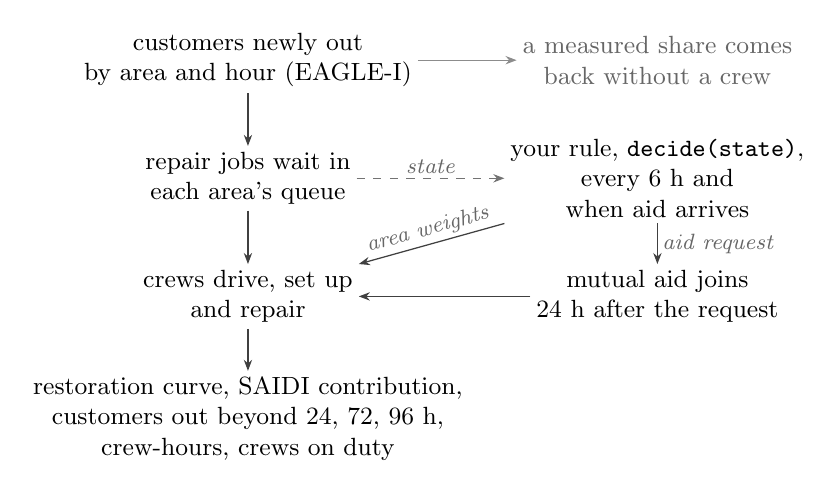
\begin{tikzpicture}[font=\small, >={Stealth[length=4pt]},
  lab/.style={align=center, inner sep=2pt}, line/.style={->, draw=black!75, line width=0.45pt},
  tag/.style={font=\footnotesize\itshape, text=black!60, inner sep=1.5pt}]
\node[lab] (dmg) at (0,0) {customers newly out\\by area and hour (EAGLE-I)};
\node[lab] (jobs) at (0,-1.5) {repair jobs wait in\\each area's queue};
\node[lab] (crews) at (0,-3.0) {crews drive, set up\\and repair};
\node[lab] (out) at (0,-4.55) {restoration curve, SAIDI contribution,\\customers out beyond 24, 72, 96 h,\\crew-hours, crews on duty};
\node[lab, text=black!60] (auto) at (5.2,0) {a measured share comes\\back without a crew};
\node[lab] (rule) at (5.2,-1.5) {your rule, \texttt{decide(state)},\\every 6 h and\\when aid arrives};
\node[lab] (aid) at (5.2,-3.0) {mutual aid joins\\24 h after the request};
\draw[line] (dmg) -- (jobs);
\draw[line] (jobs) -- (crews);
\draw[line] (crews) -- (out);
\draw[line, draw=black!45] (dmg.east) -- (auto.west);
\draw[line, dashed, draw=black!55] (jobs.east) -- node[tag, above] {state} (rule.west);
\draw[line] (rule.south west) -- node[tag, above, sloped] {area weights} (crews.north east);
\draw[line] (rule.south) -- node[tag, right] {aid request} (aid.north);
\draw[line] (aid.west) -- (crews.east);
\end{tikzpicture}
\end{document}
